\section{SchIM Implementation}
    As previously mentioned, SchIM is a PLIM module that performs a memory loop-back through the PL side similarly to \cite{PLIM20}.
    The objective of the module is to arbitrate the access of the bus to the main memory between the different cores of the PS side at the transaction level by enforcing a given policy.
    Roughly, the module receives transactions from the PS side, acknowledges them and finally repeat them with the main memory as destination.
    The exact order in which inter-core transactions are being repeated is decided by an embedded on-chip hardware scheduler.

    The present section exposes how SchIM interacts with the remaining of the systems in \ref{subsec:communication-scheme}, how its internal logic enforces transaction scheduling policies in \ref{subsec:micro-arch} and finally, an example of the transaction life cycle inside the logic is provided in \ref{subsec:transaction-life-cycle}.

    \subsection{Communication scheme}
        \label{subsec:communication-scheme}
        The exact communication scheme varies depending on whether the transaction aims at reading the main memory or writing to it as emphasised in the figures \ref{fig:Write_SchIM_communication_scheme} and \ref{fig:Read_SchIM_communication_scheme}.
        This difference between the schemes is a direct consequence of the AXI protocol \cite{ARM-AXI} used.
        As illustrated in the figure \ref{fig:Write_SchIM_communication_scheme}, the writing scheme is a simple succession of two standard AXI transactions. In fact, the actions groups $1-2-3$ and $4-5-6$ are both the succession of an address phase, followed by a data phase itself followed by a response phase.

        On the other hand, the reading communication scheme is less linear as the cores are not unloading data but rather retrieve some.
        The main difference with the writing scheme lays in the fact that the entire transaction is only partially pipelined.
        As depicted in the figure \ref{fig:Read_SchIM_communication_scheme}, steps 1 and 2 can be pipelined however, the PS is still busy waiting for the data to arrive whereas, in figure \ref{fig:Write_SchIM_communication_scheme}, once the step 3 is completed, the core can resume.

        \begin{figure}
            \begin{subfigure}{.5\textwidth}
                \centering
                \begin{tikzpicture}[scale=0.6, every node/.style={scale=0.6}]
    % States
    \draw[fill={rgb:black,1;white,7}] ( 0.0, 0.0) rectangle ( 2.0, 2.0) node[pos=.5] {PS};
    \draw[fill={rgb:black,1;white,7}] ( 4.0, 0.0) rectangle ( 6.0, 2.0) node[pos=.5] {SchIM};
    \draw[fill={rgb:black,1;white,7}] ( 8.0, 0.0) rectangle (10.0, 2.0) node[pos=.5] {Memory};
    % Edges
    % PS to SchIM Address phase
    \draw[-{Stealth}] (2.00, 1.70) -- (4.00, 1.70) node[pos=.5] {1};
    % PS to SchIM Data phase
    \draw[-{Stealth}] (2.00, 1.20) -- (4.00, 1.20) node[pos=.5] {2};
    % PS to SchIM
    \draw[{Stealth}-] (2.00, 0.30) -- (4.00, 0.30) node[pos=.5] {3};
    % SchIM to Memory Address phase
    \draw[-{Stealth}] (6.00, 1.70) -- (8.00, 1.70) node[pos=.5] {4};
    % SchIM to Memory Data phase
    \draw[-{Stealth}] (6.00, 1.20) -- (8.00, 1.20) node[pos=.5] {5};
    % SchIM to Memory
    \draw[{Stealth}-] (6.00, 0.30) -- (8.00, 0.30) node[pos=.5] {6};
\end{tikzpicture}

                \caption{The six phases required to perform a write transaction}
                \label{fig:Write_SchIM_communication_scheme}
            \end{subfigure}
            \par\bigskip
            \begin{subfigure}{.5\textwidth}
                \centering
                \begin{tikzpicture}[scale=0.6, every node/.style={scale=0.6}]
    % States
    \draw[fill={rgb:black,1;white,7}] ( 0.0, 0.0) rectangle ( 2.0, 2.0) node[pos=.5] {PS};
    \draw[fill={rgb:black,1;white,7}] ( 4.0, 0.0) rectangle ( 6.0, 2.0) node[pos=.5] {SchIM};
    \draw[fill={rgb:black,1;white,7}] ( 8.0, 0.0) rectangle (10.0, 2.0) node[pos=.5] {Memory};
    % Edges
    % PS to SchIM Address phase
    \draw[-{Stealth}] (2.00, 1.70) -- (4.00, 1.70) node[pos=.5] {1};
    % PS to SchIM
    \draw[{Stealth}-] (2.00, 0.30) -- (4.00, 0.30) node[pos=.5] {4};
    % SchIM to Memory Address phase
    \draw[-{Stealth}] (6.00, 1.70) -- (8.00, 1.70) node[pos=.5] {2};
    % SchIM to Memory
    \draw[{Stealth}-] (6.00, 0.30) -- (8.00, 0.30) node[pos=.5] {3};
\end{tikzpicture}

                \caption{The four phases required to perform a read transaction}
                \label{fig:Read_SchIM_communication_scheme}
            \end{subfigure}
            \caption{Sequence of phases in order to perform a read (a) or write (b) memory transaction from the PS to the memory by going through SchIM.}
            \label{fig:SchIM_communication_scheme}
        \end{figure}

    \subsection{Micro-architecture}
        \label{subsec:micro-arch}
        The SchIM module is composed of many sub-modules that can themselves be grouped into three different domains. In fact, as illustrated in figure \ref{fig:MemorEDF_module_schema}, one can distinguish the \emph{scheduling domain}, the \emph{queuing domain} and the \emph{interfacing domain}.

        The scheduling domain encompasses all the sub-modules that enable arbitration of the bus between the transactions issued by the different cores of the PS side. Hence, this domain boasts several transaction schedulers implemented at the hardware level.
        The scheduling policies offered by SchIM include Fixed Priority (FP), Time Division Multiple Access (TDMA), Earliest Deadline First (EDF), Least Laxity First (LLF) and MemGuard (MG).
        Each of the parameters required by the aforementioned algorithms such as the priorities, the periods, the deadlines and the budgets are re-configurable at the run-time thanks to the inclusion of a configuration port.
        Finally, the scheduling domain is also the one in charge of the control of the remaining the SchIM module, driving and selecting the adequate signals and ensuring the coherence and integrity of the data.

        The queuing domain is in charge of the storing the incoming transactions emitted by the PS side.
        The motivation behind the use of queues is implied by the fact that all the masters located on the PS side share a common AXI bus (namely HPM0 as shown in figure \ref{fig:SchIM_overview_schema}).
        Therefore, in order to cancel the Round Robin arbitration policy applied in the PS side and in order to avoid that one high priority core is stalled by a lower priority one, each core is granted a queue within the SchIM module.
        Not only the queues act as containers and buffers for transactions, they also embed logic and provide information to the scheduling domain regarding their current state in order to avoid the queues to overflow or underflow similarly to the producer-consumer problem.
        As suggested by figure \ref{fig:MemorEDF_module_schema}, transactions are inserted to the adequate queues on the basis of the emitters identifier via the dispatcher module.
        Similarly, transactions are evicted from their queue, routed by the selector module and sent directly to the output of the module upon the action of the scheduling domain.

        The interfacing domain encompasses the sub-modules in charge of interfacing both the scheduling domain and the queuing domain with the remaining of the system using the AXI protocol.
        More accurately, three sub-modules compose this domain, the configuration port previously mentioned, the packetizer and the serializer.
        While the packetizer and the serializer serve the purpose of slave and master ports, they are also in charge of respectively transforming the AXI transactions into an equivalent packet and to transform these packets back to a AXI compliant transactions.
        The need for packetizing (i.e. flattening) the AXI transactions is driven by the necessity of storing transactions that are by nature serial within the queuing domain.
        For instance, a standard AXI transaction is composed of one address phase followed by a data phase which itself composed of multiple successive bursts.

        \begin{figure}
            \centering
            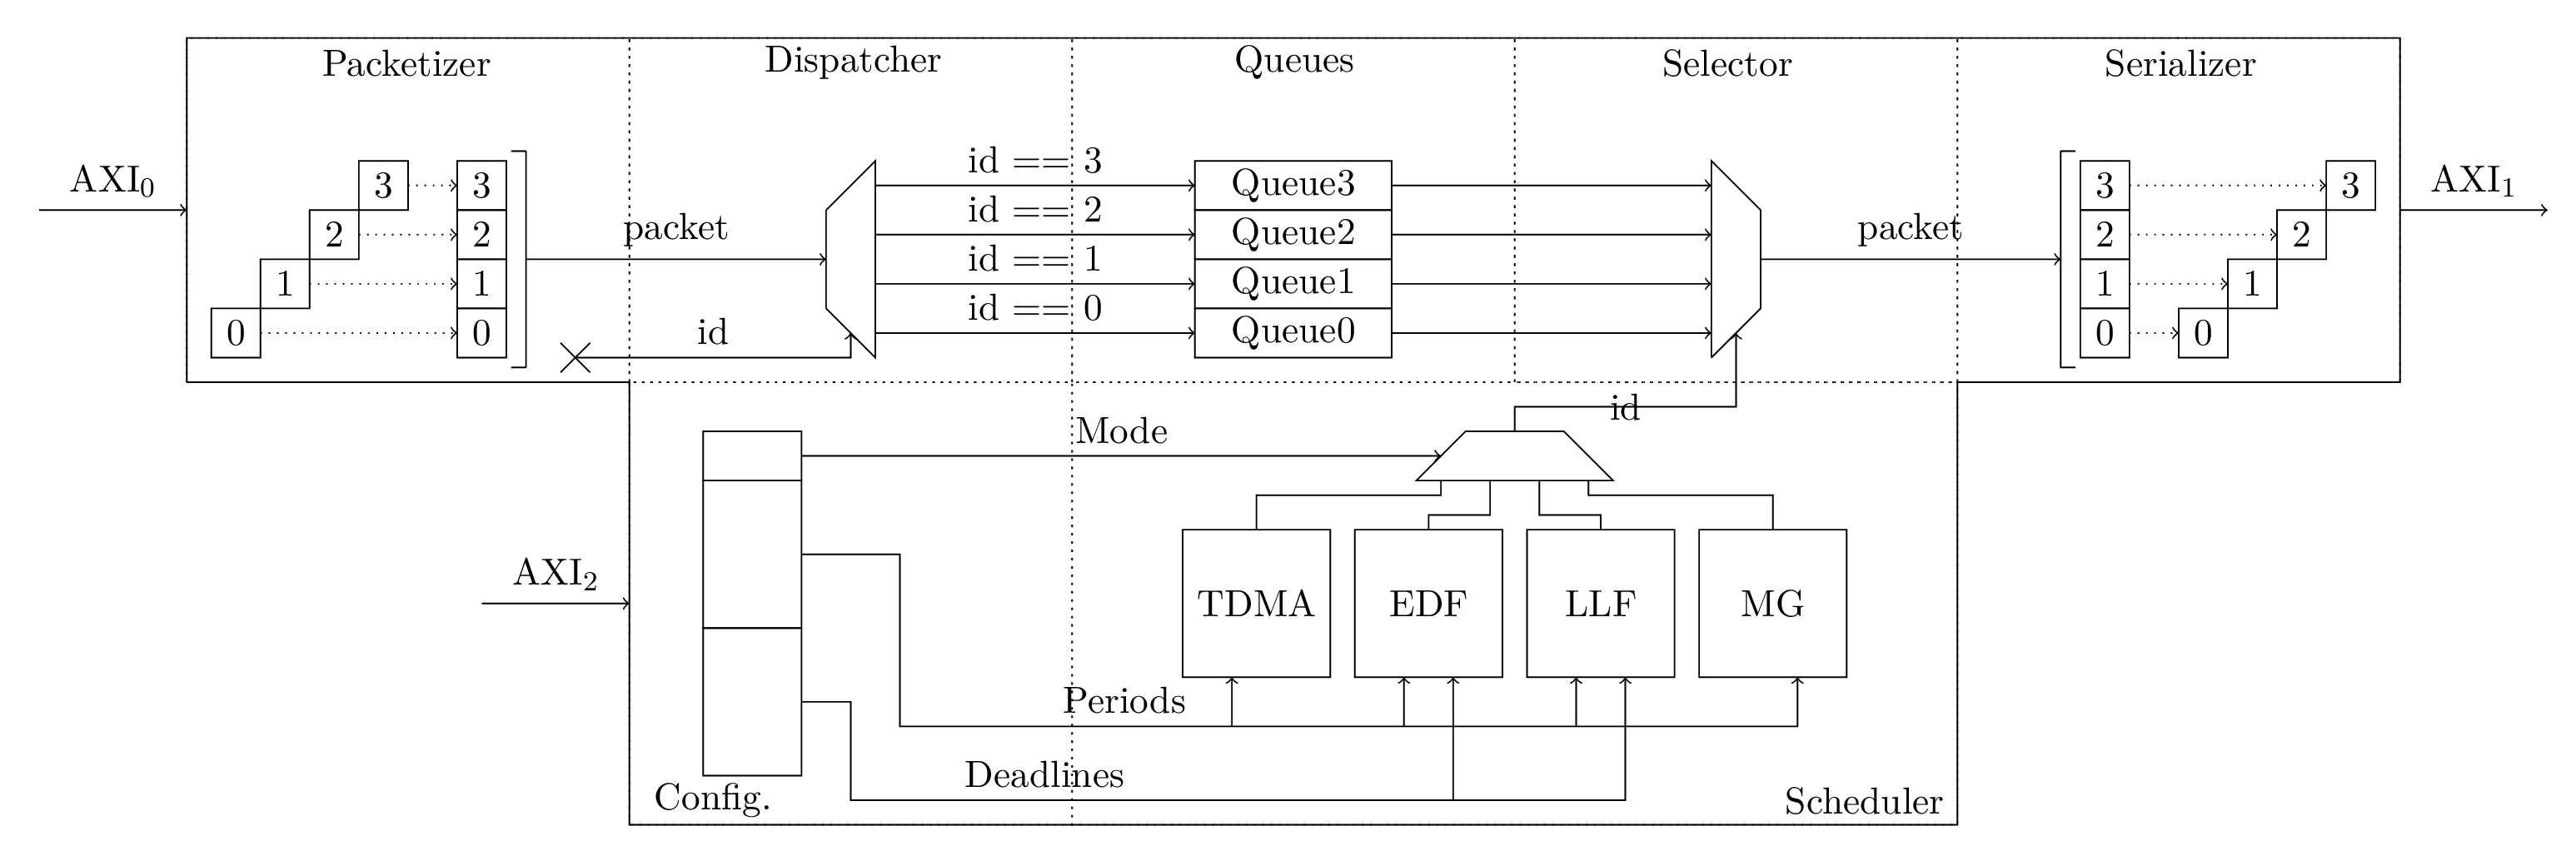
\includegraphics[scale=0.08]{images/MemorEDF_module_schema.png}
            \caption{Caption}
            \label{fig:MemorEDF_module_schema}
        \end{figure}

    \subsection{Transactions Life Cycle}
        \label{subsec:transaction-life-cycle}
        Let us consider a system with four cores (noted $C = \{c_{0}, c_{1}, c_{2}, c_{3}\}$) sending transactions $T = \{t_{0}, t_{1}, ..., t_{n}\}$ to the SchIM module.
        Consequently, the latter boasts four queues (noted $Q = \{q_{0}, q_{1}, q_{2}, q_{3}\}$) buffering the transactions under the form of packets $P = \{p_{0}, p_{1}, ..., p_{n}\}$ where $p_{i} = Packetizer(t_{i})~\forall i \in [0 : n]$.

        In the present example, we will assume $t_{1}$ as being the transaction under analysis.
        The latter is emitted by $c_{2}$ in direction of the SchIM module.
        The packetizer receives this transaction and, once the AXI protocol completed, transform it into an equivalent packet $p_{1} = Packetizer(t_{1})$.
        Following this transformation, the newly created packet is forwarded to the dispatcher which, thanks to the emitter's id embedded within the transaction, is re-routed to the corresponding queue $q_{2}$ (since emitted by $c_{2}$).
        After the insertion of $p_{1}$ in $q_{2}$, the state of the queuing domain is as follows: $q_{0}$ has two packets $p_{0}$ and $p_{k}$ and $q_{2}$ only has $p_{1}$.
        At this point, $q_{0}$ is considered for scheduling by the scheduling domain.
        In consequence, $p_{0}$ is forwarded to the serializer through the selector.
        Simultaneously to the reception of the packet by the serializer, the latter receives an activation signal from the scheduling domain informing the serializer that the packet is valid and that a transaction can be started.
        Similarly to the packetizer, the serializer will transform the packet $p_{0}$ back to its initial AXI transaction form $t_{0} = Serializer(p_{0})$.
        Thereafter, once the $t_{0}$ has been sent, the serializer will inform the scheduling domain via a signal, that he is ready to accept the next packet as input.
        Upon the reception of this signal, the scheduling domain will both re-direct the latter to the queue of the previous packet to indicate that it has been consumed and change the selected queue according to the scheduling policy so that the first packet of this queue can be forwarded to the serializer through the selector module.
        In the present example, the "consumed" signal forwarded by the scheduler is sent to $q_{0}$ which is then empty.
        At this instant, two scenarios are possible:
        \begin{enumerate}
            \item $q_{0}$ is still considered for scheduling following the selected scheduling policy. Therefore, as $q_{0}$ is empty, it outputs an "empty" signal received by the scheduling domain.
                  The latter then decides to not send any activation signal to the serializer because there is nothing left to transmit in the selected queue.
                  In other words, the access to the main memory is being stalled on purpose by the scheduling policy i.e. the scheduling policy is not work conserving.
                  For instance, such a scenario could happen in the case of TDMA or if all the queues are empty.
                  The logic will resume as soon as the selected queue is filled.
            \item $q_{2}$ is now considered instead of $q_{0}$ for scheduling.
                  In this case, the "consumed" signal is repeated to $q_{0}$ while the queue ID changes in order to select $q_{2}$.
                  This results in the packet contained inside $q_{1}$ to be forwarded to the selector.
        \end{enumerate}
